\chapter{Introduction}

This thesis seeks to explore the relationship between technological change and the recent secular increase in income inequality in Australia. We perform an empirical investigation of a number of models of technological change, beginning with the `canonical' neoclassical model of skill-biased technology. We show that skill bias does not explain empirical regularities in the wage distribution. We show that, instead, models of the task content of workers' skills, of the type proposed by \citet{Levy2003}, go some way to explaining the changing remuneration patterns of the Australian workforce.

The second half of the 20th century has witnessed tremendous change for Australian workers. Since 1973, average real per capita incomes have approximately doubled \citep{NA20124}. Economic growth has added over three million jobs to the work force \citep{LFSApr2013}. But the same period bore witness to a dramatic change in the distribution of incomes: in Australia, as well as in most developed countries, top percentile wage growth far outstripped that of lower-wage earners \citep{Atkinson1997,Borland1999,Leigh2013}. Although income inequality in Australia fell somewhat between the 1950's and 1970's, it has since risen consistently for the last 30 years, a period \citet{Leigh2013} refers to as the `Great Divergence'. \citep{Leigh2005,Gaston2009}. 

\begin{figure}[h]
  \centering
  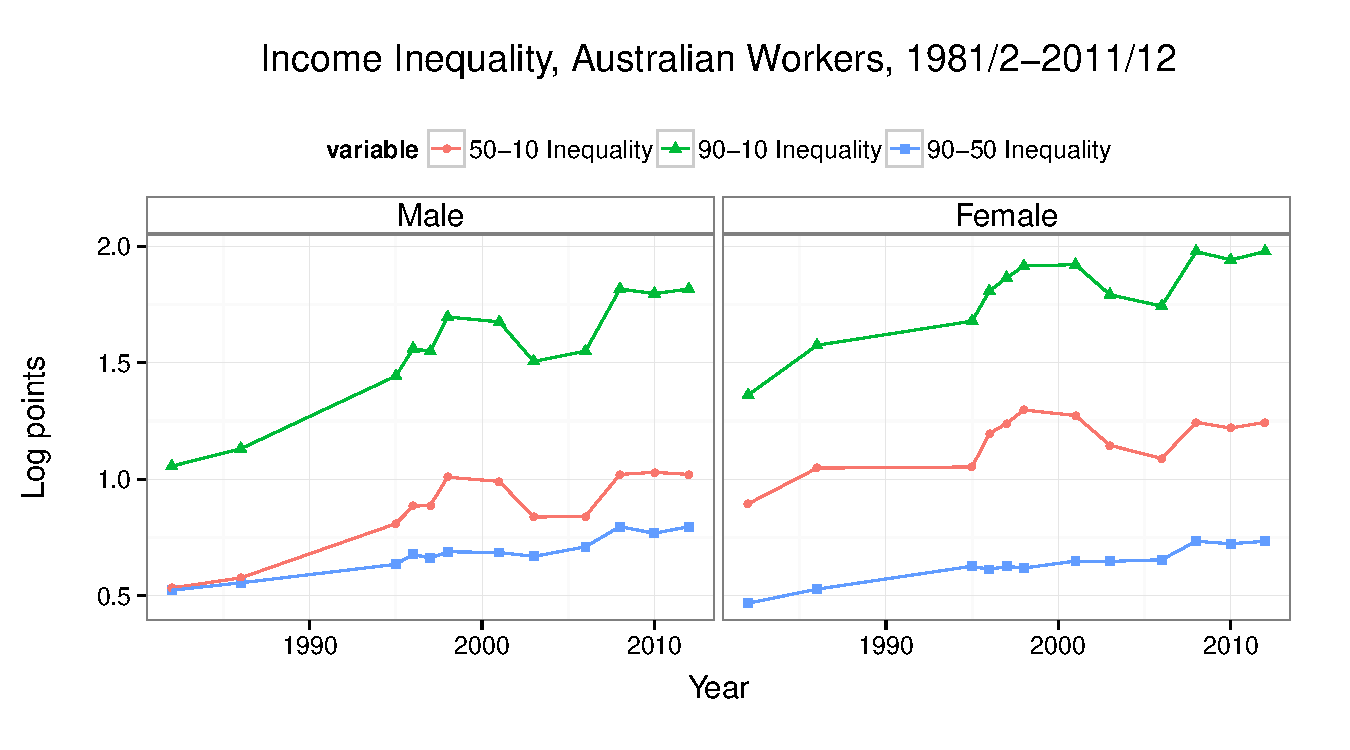
\includegraphics[width=\textwidth]{../figure/ineq_time.pdf}
  \caption{Change in income inequality measures for Australian workers, 1981/82 and 2011/12. Only workers with positive income are included, and calculations are weighted by the SIH survey weight. Source: ABS cat. 6543.0, 6541.0, 6503.0.}
\end{figure}

There is no single cause of wealth inequality, and a plurality of reasons why the total lifetime wealth of a population may diverge. In an indistrialized society such as Australia, arguably one of the most important sources of inequality is income inequality, and in particular, wage inequality is of particular importance. Figure~\ref{fig:ineq} illustrates three measures of wage inequality, over the period of the Great Divergence. During this period, 90-10 inequality grew from 1.1 to 1.8 log points for males, and from 1.3 to 2.0 log points for females. However, in recent years the causes of income inequality in Australia have been the subject of some debate.

Using cointegration techniques, \citet{Gaston2009} incorporate \citet{Leigh2005}'s income tax data in a time series model of the relationship between the Gini coefficient and macroeconomic variables, including the terms of trade, investment in ICT infrastructure, the unionisation rate, and indexes of social and economic globalisation. As well as other globalization indexes, they find that technology investment, interpreted as a proxy for SBTC, Granger (non-)causes increases in inequality, measured as the Gini coefficient.

% TODO: ACTU2012 reference below needs to be chased up
\citet{Leigh2013} names three principal causes for this surge in income inequality in Australia: falling union rates, falling income taxes and skill-biased technology. The first of these, the unionization rate, tends to reduce income inequality in the bottom of the income distribution, because they tend to bargain for across-the-board wage agreements rather than individually-negotiated employment contracts, resulting in a `compression' of the income distribution. Unions have also argued for limitations on top executive pay \citep{ACTU2012}. Any reduction in the rate of union membership therefore limits the degree of wage compression, so magnifying income inequality. This effect has been well studied elsewhere: empirical studies in the US, UK and Canada have found a signficantly negative union effect on inequality \citet{Card2004,Firpo2009}. 

The second major cause for Great Divergence is falling income taxation rates. The top marginal income tax rate in the 1908s was around 60 per cent, but this has fallen to around 40 per cent today. Consequently, the average tax rate paid by wealthy Australians has fallen, resulting in a greater divergence of accumulated wealth across the population \citet[p31]{Leigh2013}. \citet{Atkinson2013} estimate that about one third of the increase in inequality in top incomes is due to decreases in income tax.

But by far the greatest driver of increasing inequality is the inexorable rise in workplace technology. In particular, new computer and information technologies disproportionately complements skilled workers making them much more productive, but leaving unskilled workers' productivity largely unchanged. Under this model of so-called `skill biased technical change' (SBTC), new workplace technologies disproportionately complement highly-skilled technical and managerial labour \citep{Griliches1969,Autor2006}. As a result of higher productivity, wages for high-skilled jobs increase, with demand for workers outstripping the supply. Likewise, as the relative demand for lower-skilled workers has softened, so relative wage growth has stagnated. 

The three phenomena outlined above may not operate independently. \citet{Acemoglu2003} argue that skill-biased technology reduces the incentives for workers to accept the trade-off between lower wages and the improved job security and bargaining services that unions offer. If skill-biased technology improves the earnings capacity for workers with higher levels of talent or human capital, then the opportunity cost of giving up individually-negotiated contracts (where earnings may depend on that indvidual's above-average level of productivity) is considerably higher. It is thus possible that unions `amplify' inequality caused by skill-baised technical change.

The surge in inequality over the past 30 years is not a uniquely Australian experience. \citet{Atkinson2013} analyze top income rates from five Anglo-Saxon countries' tax data, and find that Australian trends described above correspond closely to the inequality patterns seen in the US, UK, Canada and New Zealand, on a wide variety of inequality measures. In all five countries, the income share accruing to the richest 0.1 per cent of income earners fell over the middle part of the twentieth century. In 1920, this group received between four and six per cent of national income (eight per cent in the U.K.), a figure that was to fall over the following half century to a nadir of around two per cent in 1980. Since the 1980s, the so-called Great Divergence has been experienced by all five countries. 

Of the many drivers of inequality, this thesis will focus on just one: the rise of skill-biased technology, and the impact of its adoption by firms. The SBTC argument, which has sparked a voluminous literature, has enjoyed considerable empirical success explaining rising wages for high-skill managerial and professional jobs in the United States and Europe \citep{Katz1992}. Since the canonical model includes \emph{factor-augmenting} capital, it predicts monotone skill upgrading of the work force at all education levels \citep{Levy2003}. Skill upgrading has been confirmed by a number of authors, both in Australia \citep{Esposto2012, Wooden2000, Cully1999} and overseas \citep{Autor2008}. 

There are good reasons for focusing on technology as a driver of changes in the work force. Although mechanical computers and computation aids (the abacus, for instance), have been available for centuries, it was only in the post-war era, with the arrival of electronic computation, that the price of computation began to fall dramatically. \citet{Nordhaus2007} estimates that, between 1946 and 2006, the cost per computation decreased by a factor of {\em seven trillion,} and over the same period, the cost of data storage fell at a comparable rate. The falling cost of computation opened up new avenues for research in information technology, so that even as computation became cheaper, new and improved algorithms were developed which made more efficient use of, and found novel uses for, computing power. And as computers have become cheaper and more useful, firms have made greater use of them. Between 1981 and 2012, Australian firms' real annual investment in computers has grown from \$26M to \$14B, in constant 2012 dollars \citet{ABS5206}.

The canonical model also predicts a rising premium for high-skill workers. In the United States in particular, SBTC has been able to explain the dynamics of the wage premium demanded by tertiary-educated labor, which fell in the 1970s and has risen in the decades to 2008 \citep{Acemoglu2011}. However, the model substantially \emph{over-predicts} the magnitude of this differential for the United States \citep{Autor2008}. In Australia, a corresponding growth in the premium for tertiary qualifications has not been observed \citep{Coelli2009}.

There are, however, a number of empirical regularities that the canonical model fails to explain. Since the late 1990s, both in Europe and the United States, the data show a marked polarization in the work force \citep{Goos2007, Autor2006}. This polarization has simultaneously manifested in \emph{wages} and in \emph{jobs}: both wage growth and growth in the level of employment are concentrated in high-skill jobs, to a lesser extent, the bottom end of the skill spectrum. Middle-skill jobs have stagnated since the 1990s, both in terms of remuneration and level.

\section{The `Task Approach'}

The neoclassical production function, which views aggregate economic output as a simple function of inputs such as capital and labor, does not consider the specifics of the processes which produced that output \citep{Acemoglu2011}. Although the canonical approach has been very successful in explaining aggregate output levels, it is not sensitive to qualitative changes in the nature of production such as changes in the technology which produce output. 

The {\em task approach}, a research program initiated by \citet{Levy2003}, presents an alternative perspective to the standard neoclassical production function. Rather than viewing output as a direct function of resource inputs, it separates the tasks performed by labor and technology, allowing  substitutions between factors \citep{Autor2013,Acemoglu2011}. 

The task approach facilitates the inclusion of worker \emph{skills} in model. For the purposes of this analysis, we follow \citet{Autor2013} in viewing a \emph{task} as a discrete unit of work, which may be used to create final goods and services, and a worker's \emph{skill}, as the stock of capabilities for the execution of those tasks. Importantly, under this framework, the allocation of workers' skills to tasks is considered endogenous to the model: heterogeneous workers apply their skills to tasks where they enjoy a competitive advantage.

Under this framework, the performance of tasks is not confined to human workers. Since the industrial revolution, investments in labor-saving capital by firms has seen a dramatic change in the performance of repetitive tasks. The pace of technical change has been continual: as automated looms replaced hand-weavers in the 18th century, so too are cheap computers replacing administrative clerks and service workers in the 21st century.

The level and price of task-performing labor can be 
viewed as an outcome of the demand for particular tasks from workers and machine capital, and the supply of task-performing labor and capital. Unlike the canonical model, where technology is viewed as factor-augmenting,  technology can therefore be viewed as substitutes for some tasks, and complements for others. Thus firms are able to substitute between capital and human workers for the execution of tasks.

\section{ICT and Routinization}

In recent decades, the most important source of labor-saving capital has been information and computer technology (ICT). As the real cost of computation has fallen precipitously over the 20th century, computers have been able to execute a wider range of tasks at a lower cost. In the presence of falling costs of ICT, the question of work force polarization can thus be framed as an outcome of a decline in the real cost of computing capital, relative to the wage cost of human workers performing similar tasks.

Computers, despite their sophistication, are only capable of performing a very limited set of simple, routine tasks. They excel at processes which require calculation and simple symbolic manipulation, and are not prone to the same types of errors as human workers. It is this fact which has led to their widespread adoption in automated tellers and a wide range of electronic service delivery which were formerly the domain of human personnel. Yet, any task that requires abstract thought or physical coordination, however elementary they may appear to a human worker, is out of reach for a computer. Activities such as stacking shelves or driving a taxi are areas in which, for the moment at least, human workers enjoy a competitive advantage \citet{Levy2003}. 

Non-routine tasks, on the other hand, may improve, rather than replace, the efficiency of human workers. Indeed, as \citet{Borland2004} found by studying the computer knowledge of a cross-section of Australian workers surveyed in 1992, computer knowledge accrues a skill premium of around 10\%.

Thus computing capital is a complement to some kinds of task-performing labor, and a substitute for others. As \citet{Levy2003} show, in the United States between 1960 and 1998, computerization led to a substitution in the observed levels of employment, away from routine tasks and toward cognitive tasks. Likewise, \citet{Goos2007} show a similar trend in the United Kingdom: between 1975 and 2003, they find a increase in the number of ``lovely'' (high-skill, high-wage) jobs and ``lousy'' (low-wage, low-skill) jobs, but a relative decrease in the number of ``middling'' jobs. In a subsequent paper, a similar pattern was found for Continental Europe \citep{Goos2009}.

It is therefore plausible, that the widespread adoption of ICT is a major driving force behind compositional changes in the workforce. 

\section{Road map and Contribution}

The rise of inequality in Australia has been well documented. Empirical studies have confirmed that both individual-level and household-level inequality have been rising since the 1980s \citep{Borland1999,Leigh2005,Leigh2013,Gaston2009}. A number of studies exist on the task content of Australian jobs \citep{Esposto2012a}, and the change over time of the skill intensity of various professions \citep{Esposto2012, Esposto2012a}. Although ICT use and globalization have been found to (non-)Granger cause rising inequality at the aggregate level \citep{Gaston2009}, no studies have tested whether workers' job types and on-the-job activities explain the nature of these changes.

In this thesis, we test the hypothesis that skill-biased technical change can explain the rise of inequality in Australia. In particular, we test whether the use of technology, in the form of ICT capital investment, automation and machinery, has displaced workers in certain kinds of jobs. And we attempt to decompose changes in the income distribution according to the type of tasks that workers perform in their jobs.

%%% Local Variables: 
%%% mode: latex
%%% TeX-master: "thesis"
%%% End: 
